\subsection{RadixSort}

\subsubsection{Ý tưởng}

Radix Sort không hoạt động bằng cách so sánh trực tiếp các phần tử với nhau như nhiều thuật toán sắp xếp khác. Thay vào đó, nó khai thác một cách tiếp cận khác: sắp xếp dựa trên các chữ số.
\begin{itemize}
    \item Phân tách theo chữ số: Radix Sort sẽ xem xét từng chữ số của các số trong dãy, từ chữ số cuối cùng (hàng đơn vị) đến chữ số đầu tiên (hàng cao nhất).
    \item Tạo các nhóm: Dựa trên giá trị của mỗi chữ số, các phần tử sẽ được phân vào các nhóm tương ứng. Ví dụ, nếu đang xét chữ số hàng đơn vị, các số có chữ số hàng đơn vị là 0 sẽ vào một nhóm, các số có chữ số hàng đơn vị là 1 sẽ vào một nhóm khác, và cứ thế.
    \item Sắp xếp các nhóm: Các nhóm này sẽ được sắp xếp lại theo thứ tự của các chữ số đang xét.
    \item Kết hợp các nhóm: Sau khi sắp xếp xong, các nhóm sẽ được kết hợp lại thành một dãy mới.
    \item Lặp lại: Quá trình trên được lặp lại cho các chữ số tiếp theo cho đến khi xét hết tất cả các chữ số.
\end{itemize}
    

\subsubsection{Các bước hoạt động}
Xét mảng A như sau: 
\begin{center}
   A = \{954, 354, 9, 411\} 
\end{center} 

\textbf{Các bước thực hiện:}

\begin{enumerate}
    \item \textbf{Xác định số chữ số lớn nhất:}
    \[
    \text{Phần tử có số chữ số lớn nhất là } 954, \text{ với 3 chữ số.}
    \]

    \item \textbf{Sắp xếp theo hàng đơn vị:}
    \begin{itemize}
        \item Lấy chữ số hàng đơn vị của mỗi phần tử:
        \[
        954 \rightarrow 4, \quad 354 \rightarrow 4, \quad 9 \rightarrow 9, \quad 411 \rightarrow 1.
        \]
        \item Sắp xếp dựa trên chữ số này:
        \[
        A = \{411, 954, 354, 9\}.
        \]
    \end{itemize}

    \item \textbf{Sắp xếp theo hàng chục:}
    \begin{itemize}
        \item Lấy chữ số hàng chục của mỗi phần tử:
        \[
        411 \rightarrow 1, \quad 954 \rightarrow 5, \quad 354 \rightarrow 5, \quad 9 \rightarrow 0.
        \]
        \item Sắp xếp dựa trên chữ số này:
        \[
        A = \{9, 411, 954, 354\}.
        \]
    \end{itemize}

    \item \textbf{Sắp xếp theo hàng trăm:}
    \begin{itemize}
        \item Lấy chữ số hàng trăm của mỗi phần tử:
        \[
        9 \rightarrow 0, \quad 411 \rightarrow 4, \quad 954 \rightarrow 9, \quad 354 \rightarrow 3.
        \]
        \item Sắp xếp dựa trên chữ số này:
        \[
        A = \{9, 354, 411, 954\}.
        \]
    \end{itemize}

    \item \textbf{Mảng kết quả:}
    Mảng đã sắp xếp:
    \[
    A = \{9, 354, 411, 954\}.
    \]

\end{enumerate}


\begin{figure}[H]
    \centering
    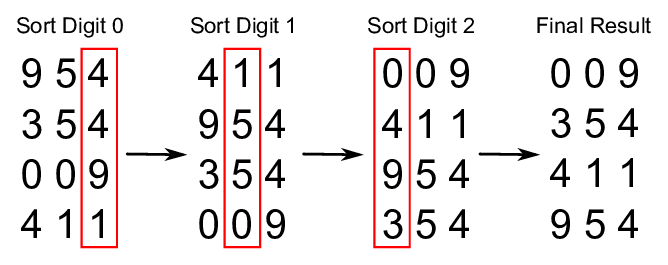
\includegraphics[width=0.8\textwidth]{img/radix.png}
    \caption{\href{https://velog.velcdn.com/images/shitaikoto/post/cc26c311-7ca9-4235-b134-27fc6480b3e9/radix.png}{Radix Sort Algorithm Diagram}}
\end{figure}

\subsubsection{Mã giả}
 
\begin{algorithm}[H]
\caption{Radix Sort}
\label{alg:radix-sort}
\begin{algorithmic}

\Require $A$ is an array of size $n$
\Function {radix-sort}{\textit{A}}
\State $max \gets$ Maximum value in $A$
\State $exp \gets 1$
\While{$max/exp > 0$}
    \Call{counting-sort}{A, exp}
    \State $exp \gets exp \times 10$
\EndWhile
\EndFunction

\Function {counting-sort}{\textit{A}, \textit{exp}}
\State Perform Counting Sort on $A$ based on the digit at $exp$ position
\EndFunction

\end{algorithmic}
\end{algorithm}


\subsubsection{Độ phức tạp}

\textbf{Độ phức tạp thời gian}

Trong cả ba trường hợp (tốt nhất, trung bình, tệ nhất), Radix sort đều cần thực hiện d bước (với d là số chữ số của số lớn nhất trong mảng). Trong mỗi bước, Counting Sort có độ phức tạp thời gian là $O(n)$. Do đó, độ phức tạp thời gian của Radix sort là $O(dn)$.

\textbf{Độ phức tạp không gian}

Radix Sort sử dụng Counting Sort trong mỗi lượt duyệt, do đó sử dụng mảng phụ để lưu kết quả, dẫn đến độ phức tạp thời gian là $O(n)$.

\subsubsection{Nhận xét}

\textbf{Tính ổn định}

Tính ổn định của Radix Sort được đảm bảo bởi cách thức hoạt động của thuật toán. Bằng cách phân nhóm các phần tử dựa trên từng chữ số và giữ nguyên thứ tự tương đối của các phần tử trong mỗi nhóm, Radix Sort đảm bảo rằng thứ tự ban đầu của các phần tử bằng nhau sẽ không bị thay đổi sau khi sắp xếp.

\textbf{Cải tiến}

Binary MSD RadixSort là một biến thể của thuật toán sắp xếp Radix Sort, được tối ưu hóa cho việc sắp xếp các số nguyên. Thuật toán này phân chia các số dựa trên từng chữ số ở cơ số 2 (hệ nhị phân) và không tốn
thêm bộ nhớ làm mảng tạm.